\section{Waveform of PMT} % (fold)
PMT is a device which is highly sensitive to even single photon. Therefore, PMT is widely used in neutrino experiments based on liquid and dark matter experiment. In neutrino experiments, liquid scintillator emits light after excited by candidate particles and charged particles emit Cherenkov light in liquid. Timing resolution is crucial in neutrino event reconstruction. 

Timing resolution is determined by PMT and waveform analysis. Typical PMT response includes 3 individual processes: photo-electron conversion happened on photocathode. Electron collection by the first dynode. And amplification of electrons between dynodes. So 1 photon incoming has a certain probability to be observed via PMT voltage(Fig \ref{fig:spe}). But if photons hit the PMT continually, the PE response will pile-up(Fig \ref{fig:pile}) and the waveform analysis will be difficult. Pile-up will significantly worsen timing resolution. 

\begin{figure}[H]
\begin{minipage}{.5\textwidth}
\begin{figure}[H]
    \centering
    \caption{PMT Single PE response}
    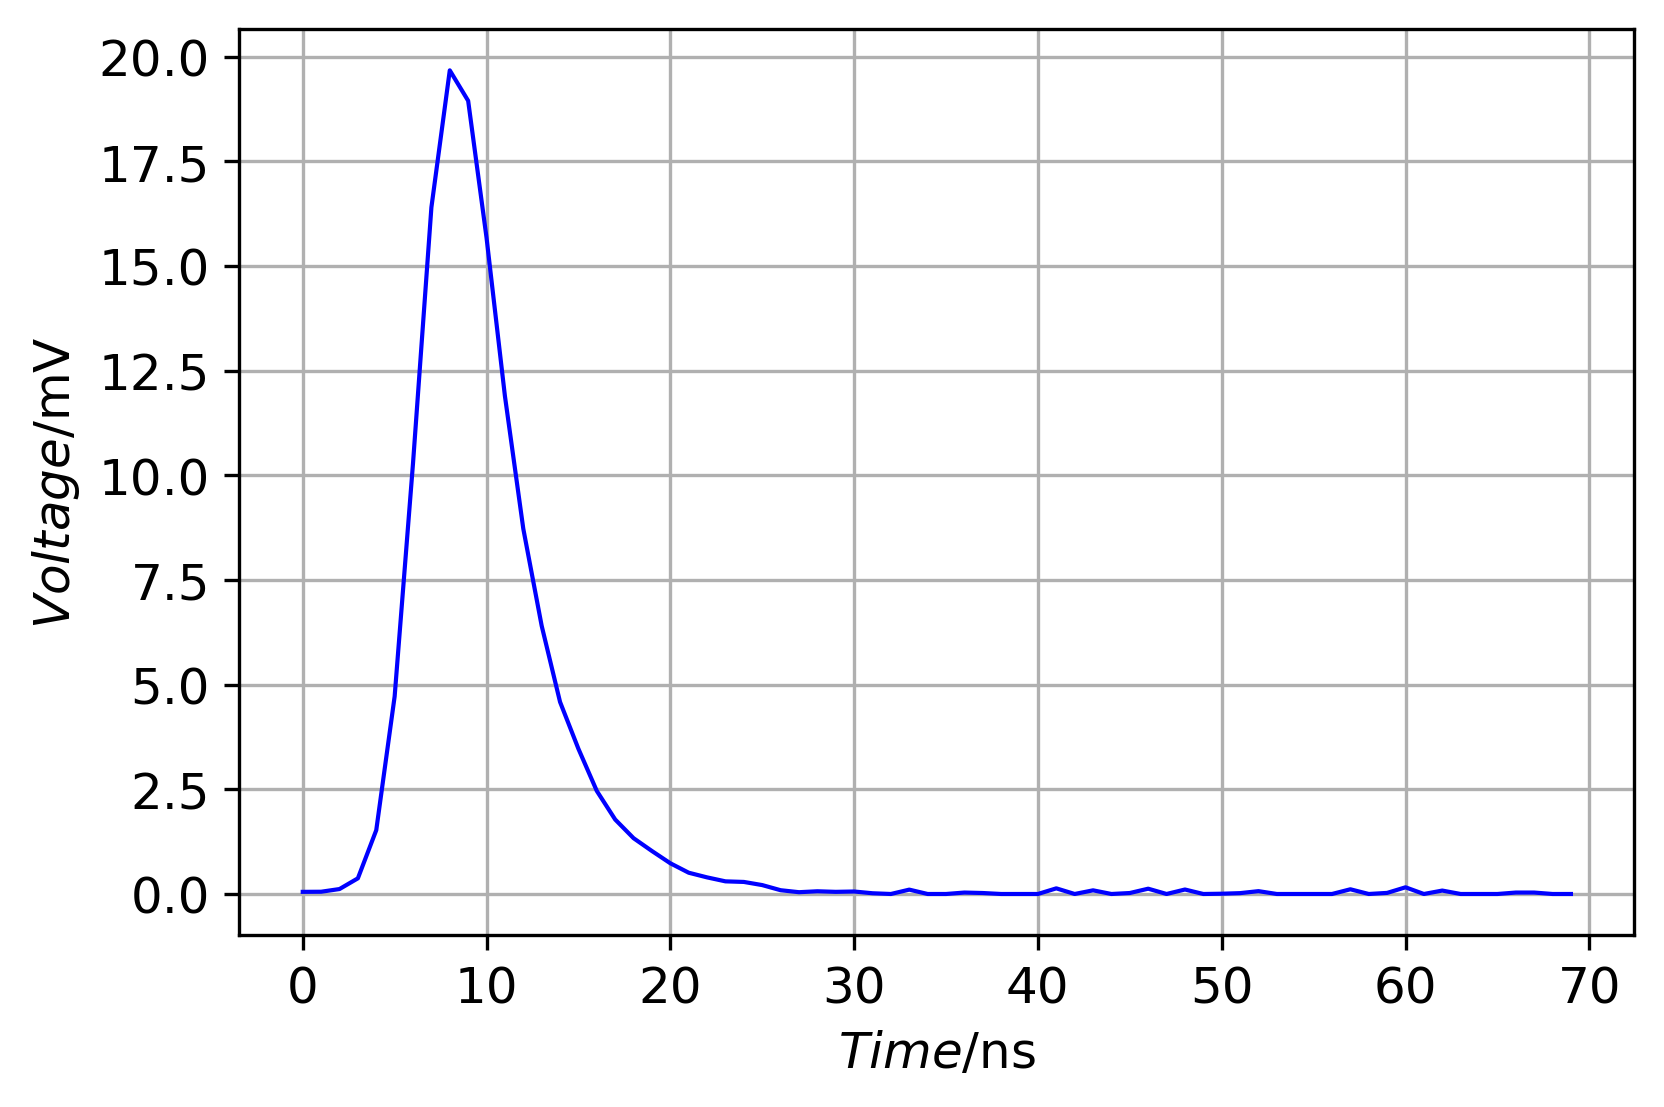
\includegraphics[width=1.0\linewidth]{figures/pmtspe.png}
    \label{fig:spe}
\end{figure}
\end{minipage}
\begin{minipage}{.5\textwidth}
\begin{figure}[H]
    \centering
    \caption{Pile-up in waveform}
    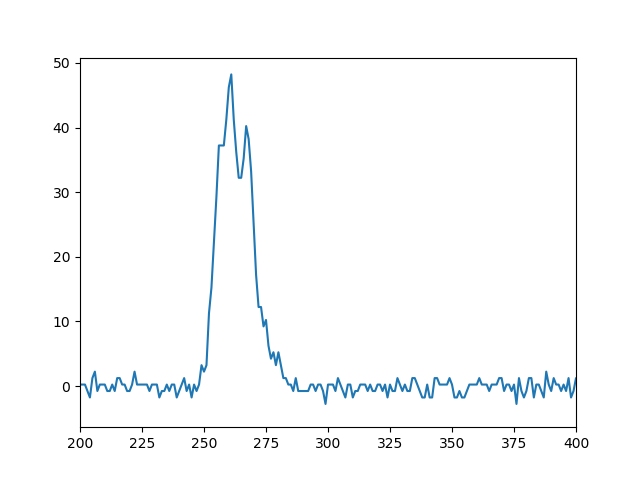
\includegraphics[width=1.0\linewidth]{figures/wave.png}
    \label{fig:pile}
\end{figure}
\end{minipage}
\end{figure}

Naively, when we handle PMT waveform we record the first hittime according to threshold and the integration of waveform. So one waveform is converted to a pair of numbers. And we lose more detailed information of the waveform(Fig \ref{fig:tradi}). The new goal is to extract information of all hits in 1 DAQ window including HitTime (the time when electron hit the first dynode) \& Charge or \#PE (number of photo-electrons)(Fig \ref{fig:new})

\begin{figure}[H]
\begin{minipage}{.5\textwidth}
\begin{figure}[H]
    \centering
    \caption{Traditional Recorded Waveform}
    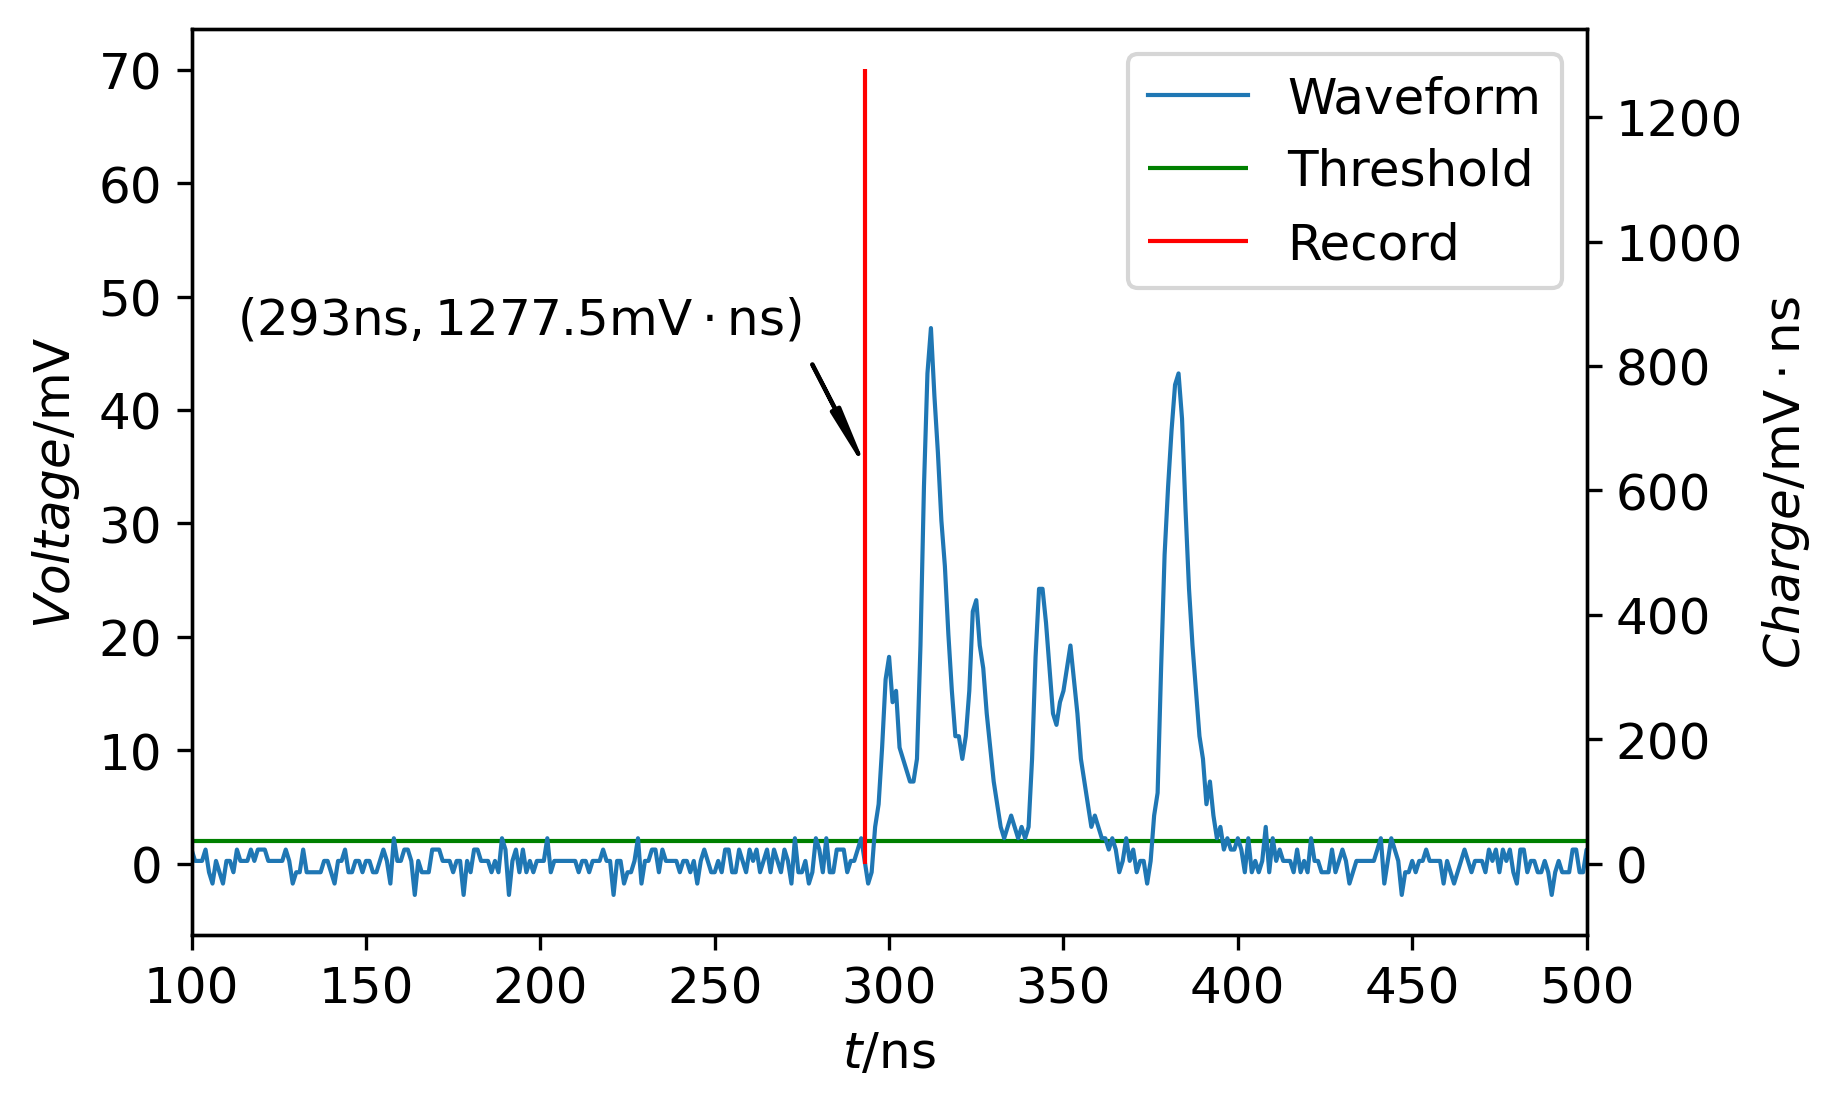
\includegraphics[width=1.0\linewidth]{figures/previous.png}
    \label{fig:tradi}
\end{figure}
\end{minipage}
\begin{minipage}{.5\textwidth}
\begin{figure}[H]
    \centering
    \caption{New Goal Recorded Waveform}
    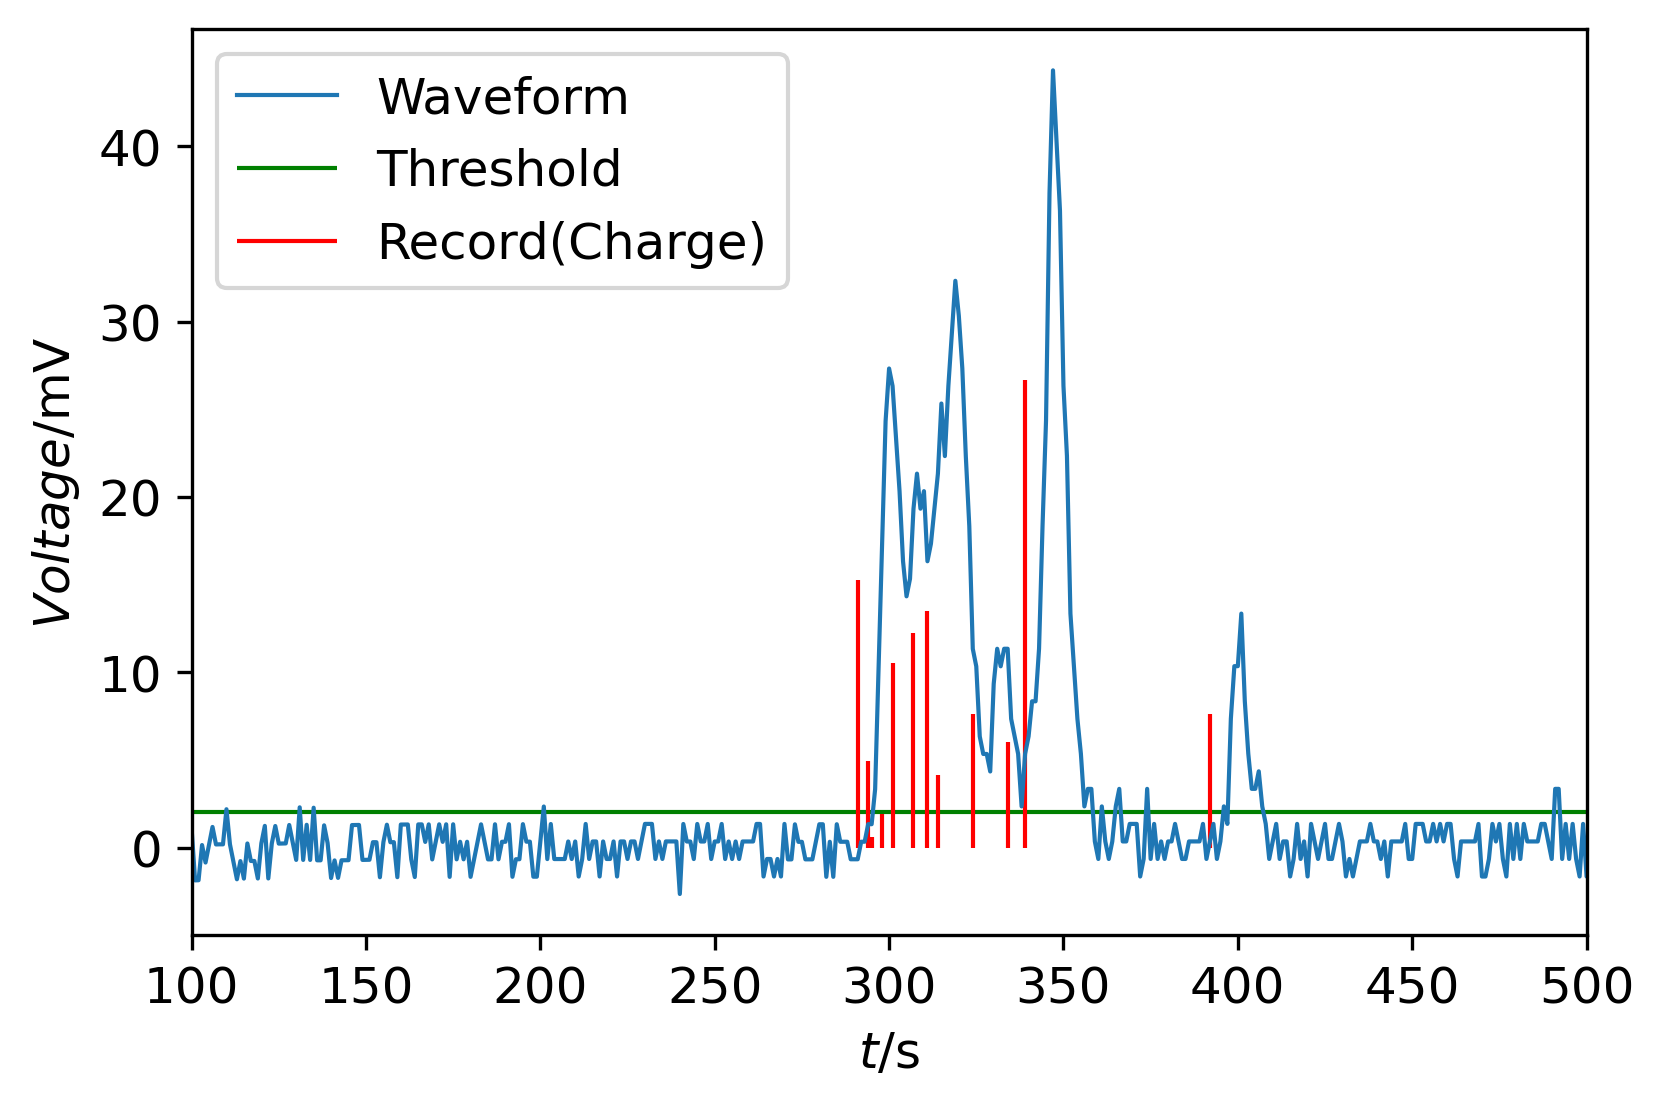
\includegraphics[width=1.0\linewidth]{figures/goal.png}
    \label{fig:new}
\end{figure}
\end{minipage}
\end{figure}

% section Waveform of PMT (end)